% This is LLNCS.DEM the demonstration file of
% the LaTeX macro package from Springer-Verlag
% for Lecture Notes in Computer Science,
% version 2.4 for LaTeX2e as of 16. April 2010
%
\documentclass{llncs}
%
\usepackage{makeidx}  % allows for indexgeneration
\usepackage{graphicx}
\usepackage{float}
\usepackage{mathtools}
\usepackage{wrapfig}
\usepackage{hyperref}
\usepackage[utf8x]{inputenc} 
\usepackage[italian]{babel} 
%
\begin{document}
%
\frontmatter          % for the preliminaries
%
\pagestyle{headings}  % switches on printing of running heads
%\addtocmark{GitHub prediction} % additional mark in the TOC

%\tableofcontents
%
\mainmatter              % start of the contributions
%
\title{Battaglia Navale multi-giocatore Distribuita}
%
\titlerunning{Battleship multiplayer distributed}  % abbreviated title (for running head)
%                                     also used for the TOC unless
%                                     \toctitle is used
%
\author{Francesco Ferretti, Di Giacinto Ettore, Andrea Iannì}
%
\authorrunning{Francesco Ferretti, Di Giacinto Ettore, Andrea Iannì} % abbreviated author list (for running head)
%
%%%% list of authors for the TOC (use if author list has to be modified)
\tocauthor{Andrea Iannì; Francesco Ferretti; Ettore di Giacinto}
%
\institute{University of Bologna, Alma Mater Studiorum, Department of Computer Science, Italy\\
\email{andrea.ianni@studio.unibo.it; francesco.ferretti10@studio.unibo.it; ettore.digiacinto@studio.unibo.it},\\
}

\maketitle              % typeset the title of the contribution

\begin{abstract}
In questo progetto è stata sviluppata una variante della battaglia navale comprensiva di $n$ giocatori, distribuita e tollerante a \emph{n-1} guasti di tipo crash. Il sistema è strutturato con un anello di comunicazione con token per l'accesso alla sezione critica dei vari nodi, che viene rigenerato in caso di perdita di nodi.
%Da modificare perché non mi viene meglio adesso
\keywords{Battaglia navale, Sistema Distribuito, Token Ring, Crash Fault Tolerance}
\end{abstract}

\section{Introduzione}
La Battaglia navale è un gioco da tavolo molto diffuso a livello globale che colloca le sue origini alla fine dell'800 e si è diffuso durante le guerre mondiali, grazie ai soldati ed ufficiali che lo usavano come passatempo.\\
Il gioco si svolge con l'utilizzo di due griglie, di dimensione solitamente 10x10; queste rappresentano i quadranti di mare del giocatore e del suo avversario. I due giocatori coinvolti, ognuno nel proprio quadrante, dispongono un eguale numero di navi (7 nel gioco classico) di varie dimensioni.\\
Il gioco procede con una serie di turni in cui ogni giocatore spara nel mare dell'avversario e questo gli risponde se il colpo è andato a segno o meno; vince il giocatore che affonda tutte le navi del nemico.
\subsection{Varianti}
Esistono molte varianti al gioco per renderlo più interessante, come ad esempio quello di non notificare l'avversario dell'esito del colpo.\\
Una variante interessante e che rende più realistico il gioco è la possibilità di poter sparare tanti colpi quanti sono le navi ancora in gioco. Quest'ultima variante è stata inclusa poi nel progetto per aumentarne la giocabilità. \\
\subsection{Stato dell'arte e obiettivi}
Data l'età e l'estrema diffusione del gioco vi sono moltissime implementazioni, dai giochi elettronici ai software online.\\
Le versioni per Nintendo DS\texttrademark ad esempio supportano schemi di gioco con griglia 8x8 e numero di giocatori pari a 4, con varie opzioni e modalità personalizzabili.\\
Un obiettivo fondamentale di questo lavoro è quello di estendere il gioco dalla modalità uno contro uno (o massimo 4 contro 4) a quella di tipo $n$ contro $n$, aumentando di conseguenza la complessità del gioco stesso.\\
Altro obiettivo è la totale distribuzione del gioco sui dispositivi dei partecipanti, che quindi dovranno gestire l'andamento del gioco e gli eventi eccezionali in maniera del tutto trasparente.\\
Il problema si può quindi tradurre come un sistema distribuito con accesso a sezione critica.\\
La memoria condivisa è rappresentata dal tabellone di gioco che viene modificato dagli utenti ad ogni turno, sparando colpi e/o affondando navi. I giocatori, inoltre, dovranno avere sempre una visione di gioco aggiornata e coerente con quella degli altri giocatori.\\
L'idea di modifica a turni dello stato globale condiviso può essere rappresentata da una struttura token ring, temporizzato che garantisce l'equo accesso alle risorse condivise.\\
Data inoltre l'imprevedibilità del comportamento degli utenti si rende necessario anche gestire eventuali eccezioni derivanti dall'uscita anticipata di un giocatore dal gioco per un qualsiasi motivo.\\
Quindi c'è bisogno di estendere le capacità della struttura token ring in modo che riesca a supportare l'uscita dei nodi partecipanti alla partita e quindi tollerare guasti di tipo crash.\\
Infine bisogna minimizzare la quantità di messaggi scambiati e le loro dimensioni per far si che non ci sia spreco di risorse e si aumenti l'efficienza del sistema.

\subsection{Struttura della relazione}
Nella parte seguente di questa relazione procederemo innanzitutto all'analisi progettuale, in cui verranno esposte le scelte effettuate per l'implementazione del software, motivandole ed analizzando gli effetti delle stesse.\\
Verranno poi discussi gli aspetti implementativi e la struttura generale del progetto.\\
Infine si valuterà l'efficacia delle soluzioni proposte ed il confronto con le soluzioni disponibili ad oggi, infine si tratterà dei possibili sviluppi e miglioramenti del gioco sviluppato.

\section{Analisi progettuale}
Passiamo ora a descrivere le scelte progettuali effettuate per rispettare i vincoli di progetto.\\
Innanzitutto, bisogna distinguere il software sviluppato in tre sistemi separati:
\begin{itemize}
	\item il sistema di comunicazione;
	\item il core;
	\item l'interfaccia grafica.
\end{itemize}
Dato che per questo progetto si è cercato di creare un forte disaccoppiamento dei componenti, passeremo ora a descrivere la struttura singolare di ogni sua parte.
\subsection{Sistema di comunicazione}
Come già accennato in precedenza, la struttura di comunicazione ipotizzata e realizzata durante lo svolgimento del progetto è quella dell'anello con passaggio di token.\\
Questo perché la strutturazione a turni rispecchia il passaggio del token per la modifica dello stato condiviso.\\
La comunicazione ad anello è una tipologia di comunicazione molto comune nelle reti di computer, definito dallo standard IEEE 802.5 per le comunicazioni su rete locale LAN.\\
Primo problema però di questa struttura di comunicazione è l'identificazione dei partecipanti, per la creazione si è resa necessario infatti l'introduzione di un server che si occupasse di creare una stanza di gioco in cui gli utenti venissero raccolti.\\
Ogni istanza del gioco può connettersi semplicemente al server centrale, questo registra la connessione, quando si è raggiunto il numero desiderato si può avviare la partita.\\
Dato che però l'obiettivo è quello di creare un sistema completamente distribuito ne conseguirà che il server non sarà incluso più attivamente nella computazione o nella gestione dei messaggi. Quindi una volta messi in comunicazione tutti i giocatori, questi comunicano tra di loro autonomamente.\\
Dopo che gli utenti sono stati messi in contatto, bisogna organizzare l'anello in base alla lista dei partecipanti che viene fornita a tutti dal server. Questo è stato effettuato organizzato ordinando secondo uno schema prefissato la lista degli utenti, così da avere una lista identica su ogni istanza.\\
Creato l'ordinamento, ogni nodo comunicherà solo con il successivo ed il precedente, veicolando in questa maniera tutti i suoi messaggi al resto della rete.\\
Ogni volta che un utente ha il token è autorizzato a modificare lo stato globale del sistema; questo però fino a che l'utente non esce dalla rete di comunicazione. In questo caso specifico, il giocatore che ha perso tutte le proprie navi è autorizzato a controllare l'andamento del gioco ma non deve avere più la possibilità di interagire con gli altri utenti.
\subsubsection{Eventi eccezionali}
Come abbiamo già accennato il software deve adattarsi ad eventi particolari quali la caduta di un nodo della rete.\\
Nelle strutture ad anello su reti locali LAN si riescono a tollerare solamente un guasto, invertendo il verso di passaggio del token. In questo caso però non è possibile invertire il verso di passaggio del token poichè influenzerebbe le dinamiche di gioco.\\
Si è quindi scelto di modificare la struttura ad anello di comunicazione per renderla tollerante ai guasti tramite la possibilità di cambiare il collegamento al nodo successivo ogni volta che si rileva il guasto di un nodo.\\
\subsection{Core}
Il Core è il sistema che si occupa della logica di gioco, interfacciandosi al sistema di comunicazione per inviare i messaggi agli altri nodi e all'interfaccia grafica per interagire con l'utente.\\
In questa parte deve essere memorizzato lo stato globale del gioco, così ogni nodo ha una replica esatta di ciò che è accaduto durante i precedenti turni. Ogni nodo però conosce lo stato globale aggiornato all'ultima volta che il token ha transitato per lo stesso, quindi solo dopo un giro completo dell'anello il nodo conoscerà l'effettiva situazione.\\
Quindi lo stato può essere associato ad un entità che d'ora in avanti chiameremo \emph{oceano}. L'oceano corrisponde al tabellone di gioco, che quindi ad ogni mossa dell'utente viene modificato in locale e viene  propagato ad i successivi nodi dell'anello.\\
L'invio di tutto lo stato globale è però costoso, quindi si è deciso che questo venga condiviso all'interno dell'anello solo una volta durante il posizionamento delle navi,  effettuando due giri dell'anello quando tutti i giocatori hanno posizionato le navi, al fine di garantire che tutti abbiano lo stesso stato condiviso.\\
Durante le fasi successive di gioco l'entità che viene scambiata sono le coordinate dei colpi di ogni giocatore. Inviando però solo i colpi sparati all'interno del token si viene a ridurre l'effetto Real Time del sistema, che quindi risulta de-sincronizzato fino a che non avviene il passaggio dello stesso per la seconda volta. Per una migliore esperienza di gioco si è quindi scelto di far girare all'interno dell'anello i messaggi di colpi sparati dei giocatori.\\
I nodi effettuano quindi una modifica anticipata dello stato globale, prima di ricevere effettivamente il token, ma registrano definitivamente queste solo dopo averlo ricevuto con la lista di mosse.\\
\subsubsection{Eventi eccezionali}
In caso un nodo non risponde più durante la partita, questo viene rimosso dal core dalla lista di giocatori attivi, e quindi le sue navi non vengono più conteggiate tra quelle raggiungibili/affondabili.
\subsection{Interfaccia grafica}
In questa parte del progetto si effettua semplicemente l'interazione con l'utente, riportando graficamente i vari cambiamenti effettuati allo stato dagli altri giocatori e dal giocatore corrente.\\
Le azioni principali che possono essere effettuate sono il posizionamento delle navi e il fuoco sulle posizioni nemiche.\\
L'interfaccia deve anche permettere la visualizzazione degli stati di gioco per gli utenti che hanno perso e notificare questo stato a tutti gli nodi coinvolti.
\subsubsection{Eventi eccezionali}
L'interfaccia deve tenere conto di eventuali crash da parte di altri nodi, disabilitando su notifica del core tutte le aree associate a questi ultimi.	

\section{Aspetti implementativi}
Passiamo ora agli aspetti implementativi dell'architettura sviluppata, entrando più nel dettaglio della struttura del codice. Come nella parte precedente possiamo dividere la trattazione nelle tre parti sopra delineate.\\
\subsection{Comunicazione}
In questa parte ci occuperemo della descrizione dell'implementazione del sistema di comunicazione, di cui vediamo uno schema delle classi nel seguente diagramma.\\
\begin{figure}[H]
\centering
    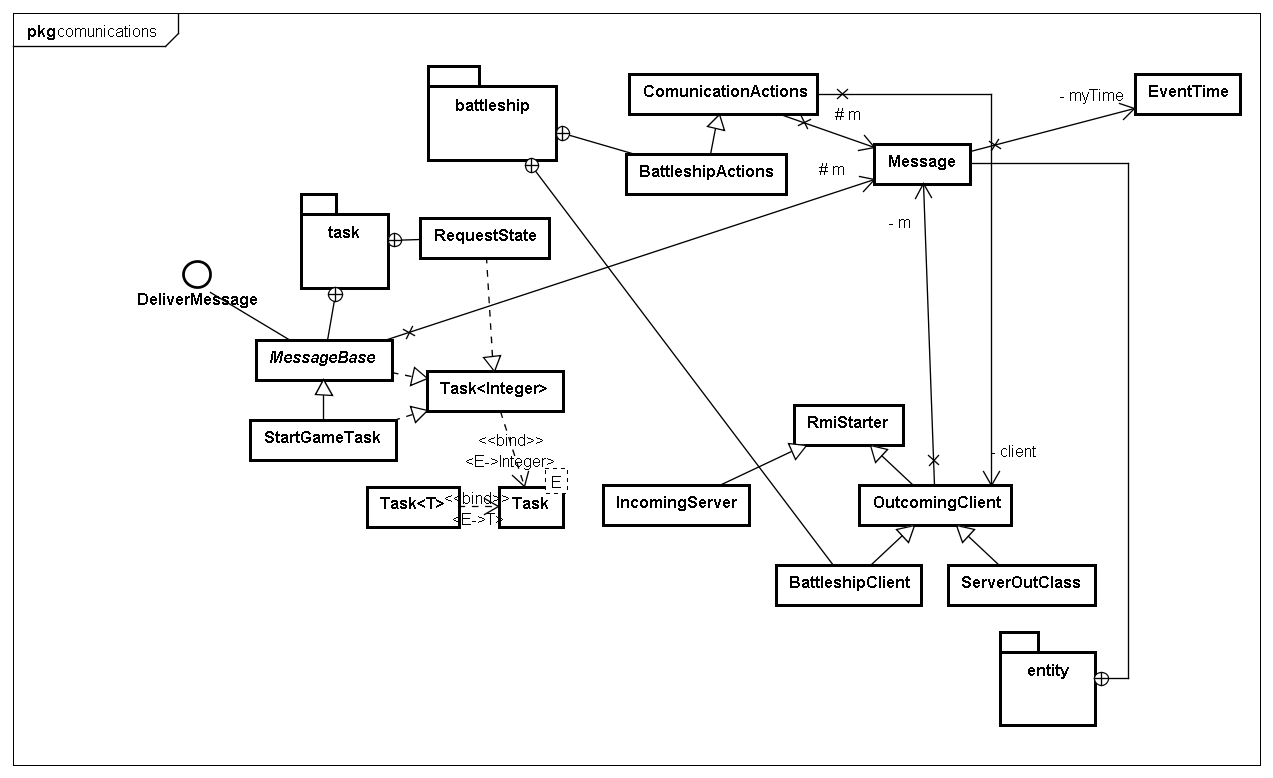
\includegraphics[width=12cm]{imgs/diagramma-delle-comunicazioni.png}
     \caption{Diagramma delle Classi dei messaggi}
   \label{output:blacknoxis_normal}
\end{figure}
Il sistema è stato sviluppato in Java, e mette in comunicazione i nodi in maniera distribuita grazie a Java RMI.\\
Remote Method Invocation è una tecnologia di Java che permette la comunicazione tra due nodi, un server ed un client. Il client effettua la richiesta di eseguire una chiamata ad un metodo remoto di una classe sul server, questo processa la richiesta e restituisce un risultato al chiamante.\\
Come si può notare dal diagramma delle classi, tutto è collegato all'RMI starter. Questo è un package da cui vengono estese le due classi principali, \emph{Outcoming Client}, di cui ci possono essere diverse istanze, e \emph{Incoming Server} di cui vi è solo un istanza. Queste due classi si occupano di fare il dispatch dei messaggi ai nodi coinvolti nella comunicazione. \\
Ad ogni comunicazione viene inviato un messaggio con la classe di tipo \emph{Message}, che estende \emph{Message Base}, il quale viene consegnato al nodo successivo.\\
Ad ogni messaggio il server successivo esegue un task ad esso associato, che corrisponde ad una determinata azione da compiere nello stato del gioco o per cambiare la topologia della rete di comunicazione.\\
Come si può notare nel seguente diagramma esistono diverse tipologie di azione associate al messaggio:
\begin{figure}[H]
\centering
    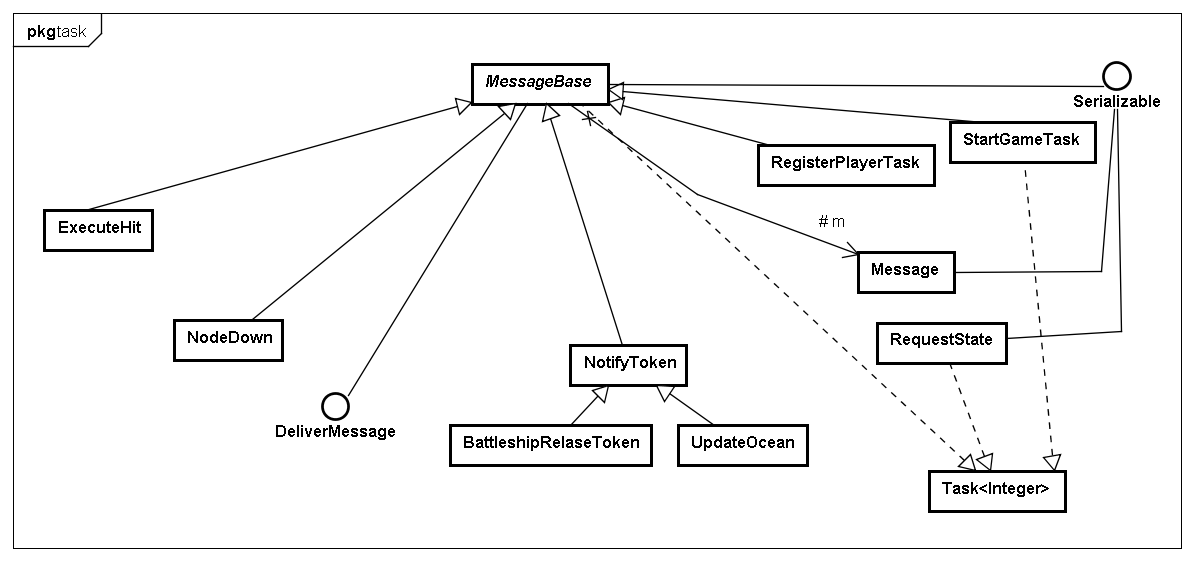
\includegraphics[width=12cm]{imgs/Task-diagram.png}
     \caption{Diagramma dei task}
   \label{output:blacknoxis_normal}
\end{figure}
Tutti i messaggi, per essere trasferibili, devono essere serializzabili, dunque implementano l'interfaccia Serializable del Java utilizzando il metodo \emph{DeliverMessage} per spedire il messaggio.\\
Ad ogni messaggio è associato un task specifico che può essere:
\begin{itemize}
	\item registrare un giocatore;
	\item iniziare il gioco;
	\item colpire una posizione della griglia;
	\item acquisire il token;
\end{itemize}
Questi task permettono la comunicazione nell'anello e il gioco in condizioni normali.\\
In caso però di caduta di un nodo bisogna attivare una serie di routine specifiche per effettuare la modifica trasparente della topologia dell'anello di comunicazione.\\
Per controllare che tutti i nodi siano presenti all'interno della corrente sessione di gioco, si utilizza un messaggio temporizzato che viene dal nodo precedente nella lista al successivo. Quindi a cascata tutti i nodi della rete controllano se gli altri partecipanti sono ancora in gioco.\\
Non appena uno di questi nodi non risponde nello slot di tempo concesso, vengono eseguiti i passi come visualizzato nel seguente diagramma di sequenza:
\begin{figure}[H]
\centering
    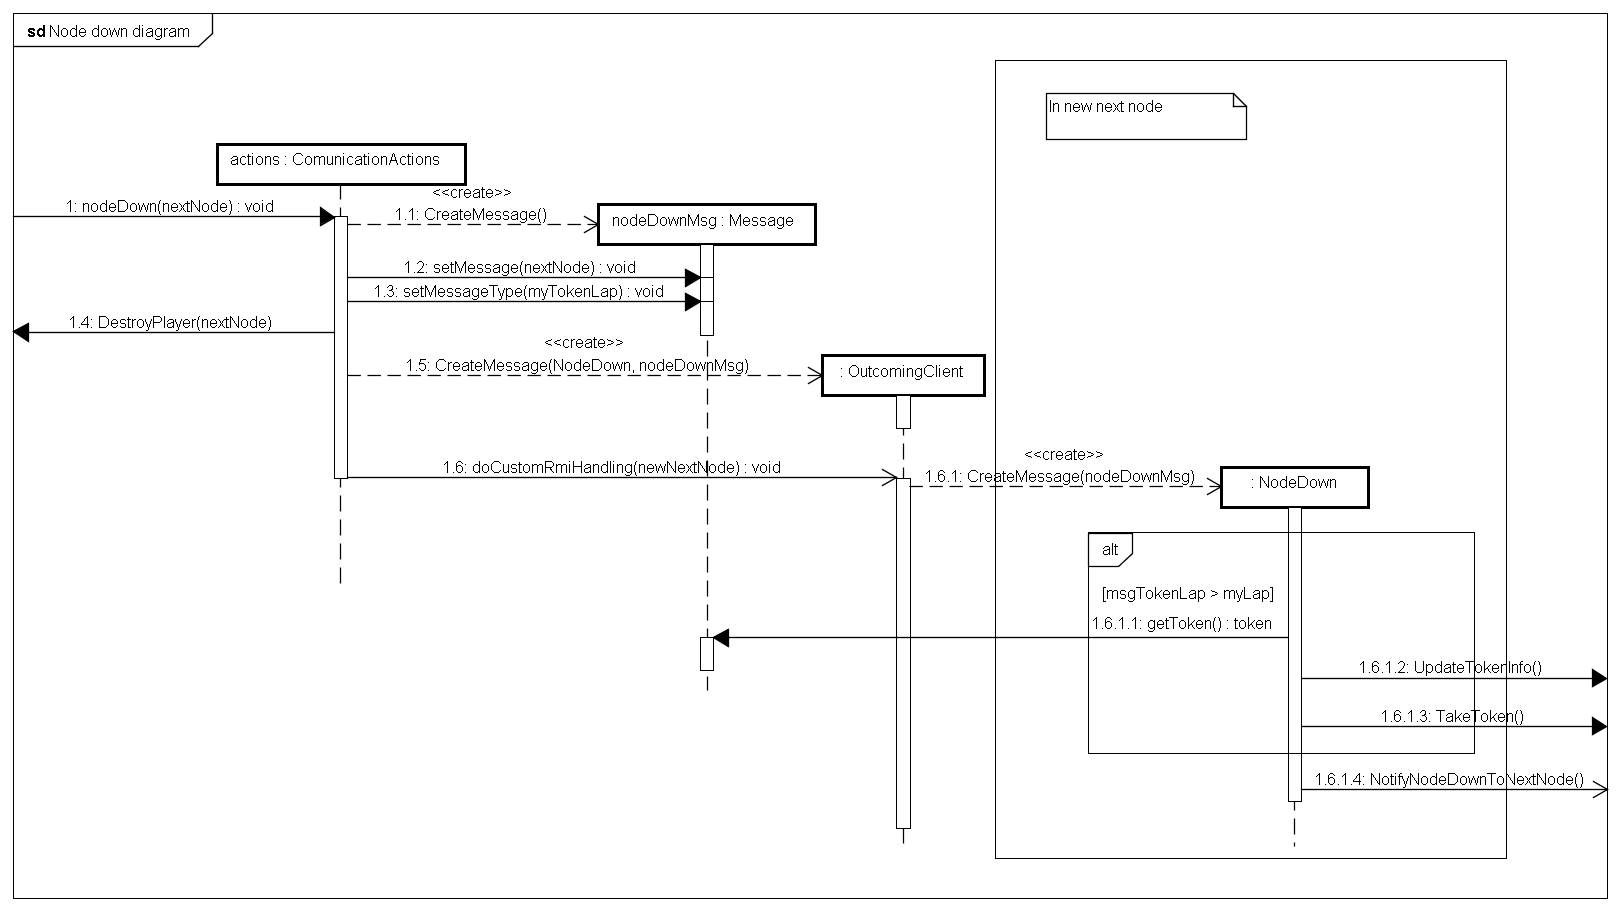
\includegraphics[width=12cm]{imgs/Node-down-diagram.png}
     \caption{Diagramma di sequenza per il nodo caduto.}
   \label{output:blacknoxis_normal}
\end{figure}
Quando un nodo si accorge che il successivo è caduto, questo esegue la ricerca del primo nodo successivo ancora online. Quando questo viene identificato genera un messaggio di \emph{NodeDown} in cui include il numero di volte che il token ha transitato per quel nodo.\\
Questo messaggio viene spedito al nodo successivo, il quale si occupa di controllare se il numero di giri che ha effettuato il token sono minori rispetto a quelli rilevati dal nodo che ha segnalato il crash. In questa maniera viene recuperato il token e ripristinate le mosse effettuate se questo è stato perso tra i nodi caduti, oppure modificando solo la topologia della rete se il token era già passato oltre.\\
Infine il nodo manda in avanti la notifica di nodo caduto all'interno della rete per far si che a tutti gli utenti venga notificata la scomparsa di un giocatore.\\
\subsection{Core}
Passiamo ora più nel dettaglio a definire la struttura del core. Questa parte del software si occupa della logica di gioco utilizzando in maniera trasparente il canale di comunicazione e ignorando la topologia della rete.\\
Di fatti l'unico collegamento con lo strato più basso del sistema è la lista dei giocatori, la quale serve solo per una disposizione delle informazioni all'interno della nostra memoria.\\
Di seguito è stato introdotto un diagramma delle classi che si occupano della logica di gioco.
\begin{figure}[H]
\centering
    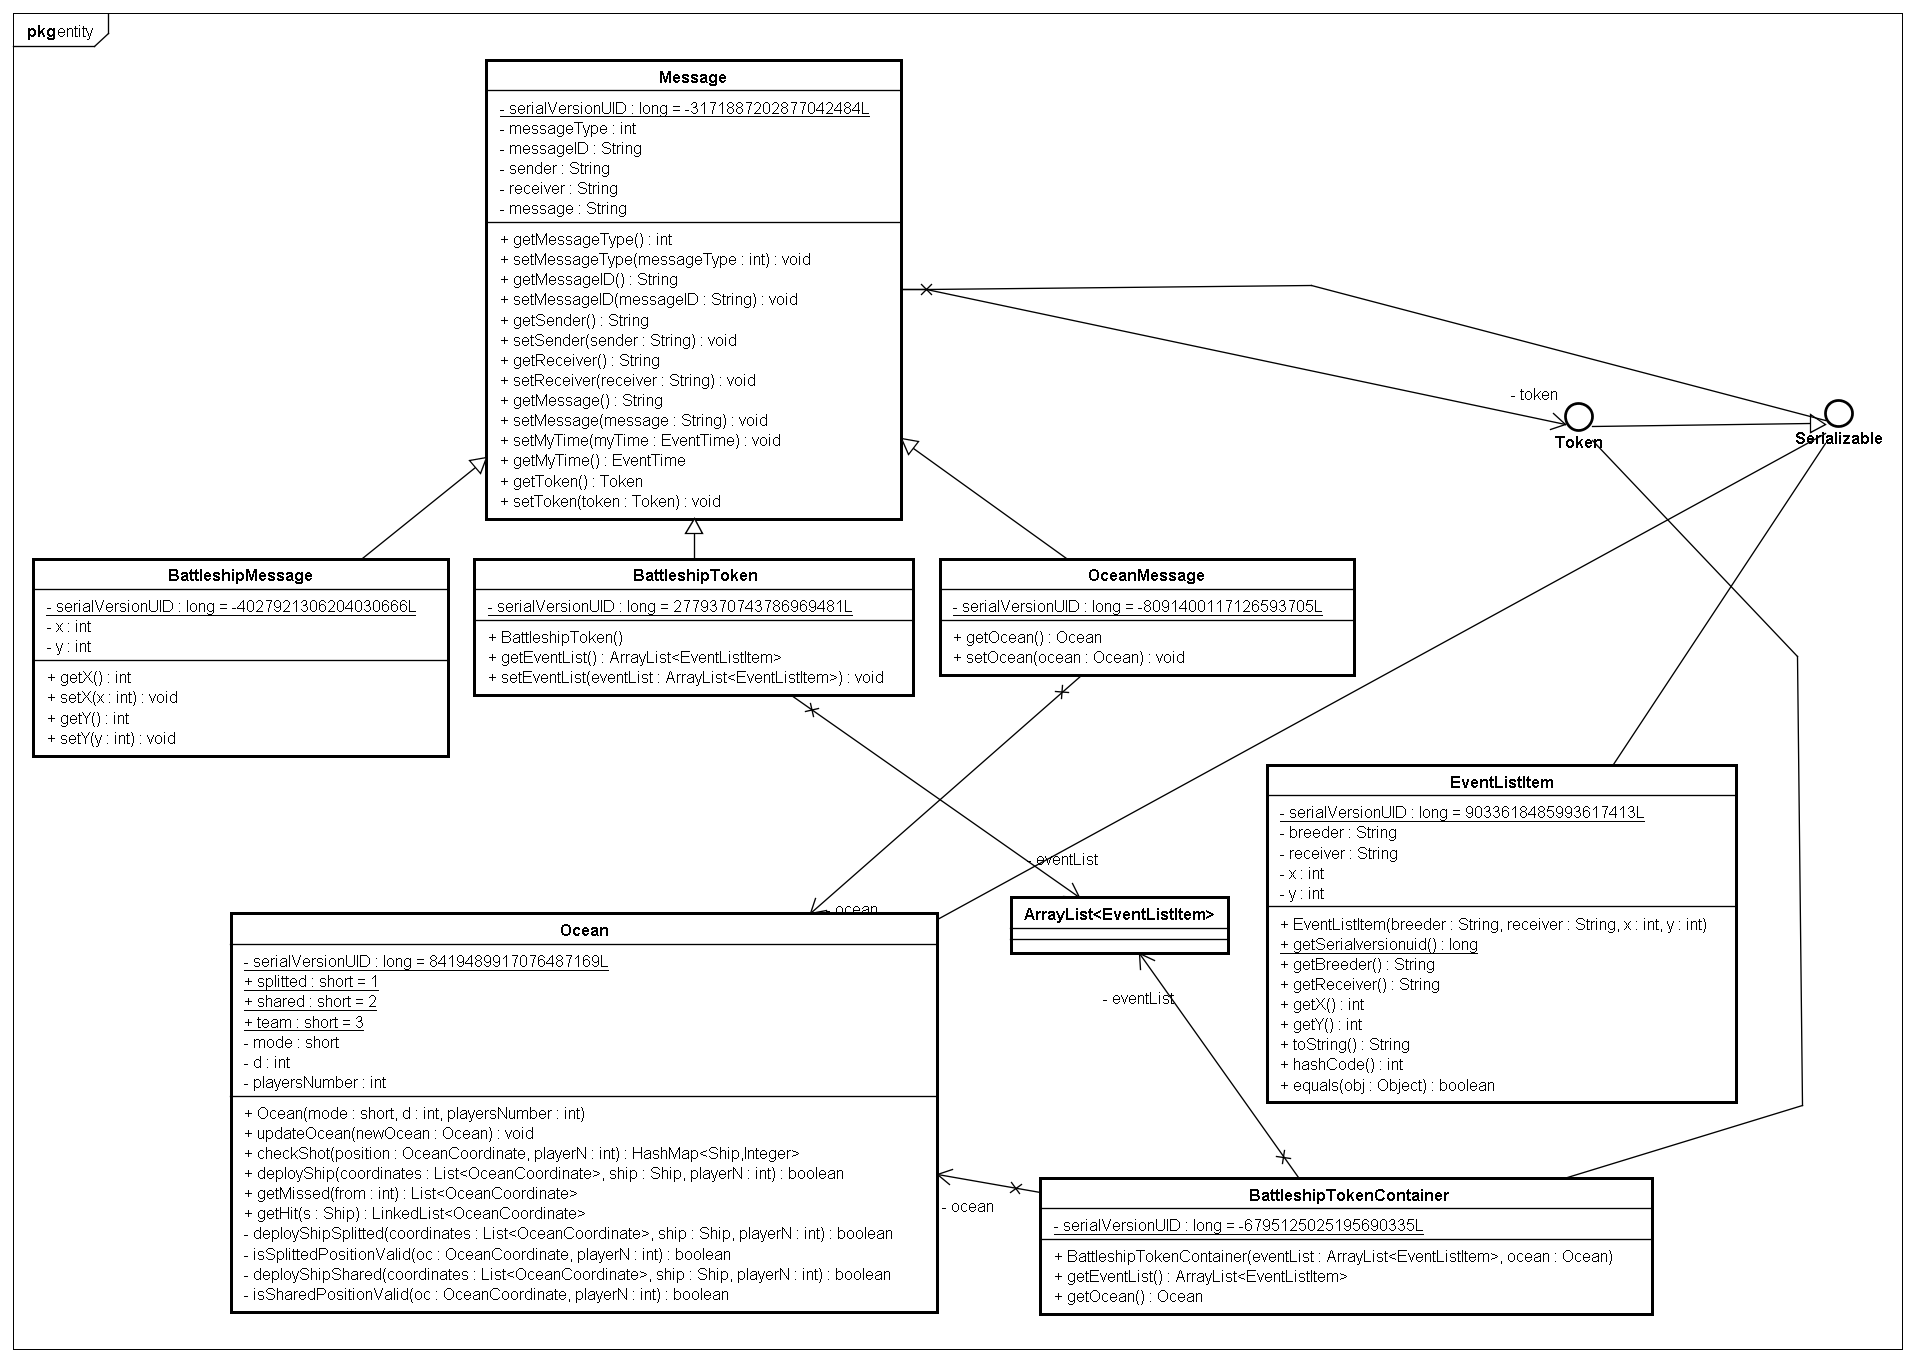
\includegraphics[width=12cm]{imgs/BattleshipMessageDiagram.png}
     \caption{Diagramma delle Classi dei messaggi}
   \label{output:blacknoxis_normal}
\end{figure}
La strutturazione fa si che l'oggetto condiviso principale sia l'oceano. Questa classe si occupa di memorizzare gli eventi e le interazioni del giocatore locale e di quelli generati dagli altri nodi della rete in una struttura dati, che mantiene una correlazione tra le navi presenti all'interno del mare e le caselle occupate.\\
Con questo metodo si minimizza l'occupazione di memoria, in favore anche di un più facile accesso alle posizioni delle navi.\\
Quando le navi vengono posizionate, queste vengono registrate all'interno della struttura dati, che in fase di boot viene condivisa nel token agli altri giocatori, in modo tale che tutti abbiano la conoscenza globale del tabellone di gioco.\\
Dopo questa fase di boot, il gioco inizia condividendo con gli altri nodi la lista di mosse effettuate da ogni giocatore; viene inserita nel token, che viene fatto ciclare all'interno dell'anello e tutti aggiungono i propri colpi.\\ 
Contemporaneamente a questa operazione avviene lo scambio del messaggio Real Time, per mezzo della classe \emph{BattleshipMessage}. La classe serve a notificare anticipatamente la modifica allo stato globale ma non è la modifica definitiva dello stato, che viene effettuata solo dopo la ricezione del token.\\
Ad ogni colpo ricevuto viene effettuato il controllo della presenza delle coordinate all'interno dell'oceano e, se queste sono presenti, vengono date per colpite tutte le navi che si trovano all'interno della posizione indicata oppure la mossa viene inserita tra i colpi mancati.\\
Una volta terminate le navi il giocatore, non uscendo dall'anello, è in grado di controllare l'andamento del gioco, ma non gli viene più permesso di effettuare modifiche allo stato globale del gioco, effettuando perciò immediatamente il release del token.\\
\subsection{Interfaccia grafica}
%Non so se dire qualcosa qui

\section{Valutazione}
Per valutare le performance del software sviluppato bisogna guardare il costo computazionale e quello dei messaggi che vengono richiesti dal sistema.\\
\subsection{Costo dei messaggi}
L'anello è una strutturazione particolare dove i messaggi richiedono, per effettuare un giro completo, il passaggio attraverso $n$ nodi differenti.\\
Nella fase di avvio del gioco, ovvero quando avviene la disposizione di messaggi, viene richiesto che si effettuino due giri dell'anello per notificare a tutti i partecipanti la posizione delle navi e quindi condividere tra tutti il tabellone di gioco.\\
Similmente durante la partita i messaggi devono effettuare un giro completo per garantire che tutti i giocatori abbiano ricevuto la modifica dello stato di gioco. Quando un nodo riceve di nuovo la sua lista di mosse, vengono cancellate quelle precedenti ed aggiunte in coda le nuove, di modo da ridurre la dimensione della lista ad un massimo di $n*s$, dove $n$ è il numero di giocatori in partita e $s$ è il numero di colpi che ogni utente al massimo può sparare.\\
In più se le mosse venissero condivise solo tramite il token, si introdurrebbe un ritardo nell'aggiornamento dello stato globale del gioco proporzionalmente grande al numero di giocatori ed al tempo che questi impiegano per effettuare una mossa.\\
Dato che questo dal punto di vista utente è inaccettabile si è scelto di introdurre un ulteriore messaggio (\emph{BattleshipMessage}) che pur generando duplicazione dell'informazione, mantiene aggiornato l'utente sullo svolgimento del gioco.\\
Infine la possibilità per i giocatori perdenti di visualizzare i processi di gioco introduce un ulteriore ritardo, in questo caso però molto trascurabile per via del fatto che il token viene solo controllato per acquisire lo stato globale del gioco e viene subito rilasciato.
\subsection{Costo computazionale}
Il gioco effettua controlli all'interno dell'oceano in $O(1)$ visto che può effettuare la ricerca e la rimozione all'interno della struttura dati che contiene le posizioni delle navi con quell'ordine di grandezza grazie all'ausilio di una HashMap.\\
Questo permette di molto di velocizzare l'esecuzione del codice dato che è l'operazione più costosa e ripetitiva di tutto il core.\\
Questo però implica che vi sia una concordanza di tutti i nodi all'interno della rete sullo stato globale, è quindi molto importante che il token arrivi integro ad ogni nodo senza alcun tipo di alterazione. 
%Qua bisognerebbe aggiungere qualcosa riguardo altre soluzioni da lui spiegate
\section{Conclusione}
In questa relazione si è discusso dell'implementazione di una battaglia navale ad $n$ giocatori, con un sistema completamente distribuito, se non per il server di boot.\\
Sono state discusse le implementazioni e struttura del canale di comunicazione e del core del sistema, con una accenno alla struttura dell'interfaccia.\\
Si è infine valutata il costo computazionale e di comunicazione del software sviluppato.\\
Il software è ancora acerbo dal punto di vista dell'interfaccia utente, ma ha un core solido e forti possibilità di espansione, che ci fanno ben sperare per ulteriori sviluppi futuri.
\subsection{Sviluppi Futuri}
Il software è stato predisposto fortemente disaccoppiato per permettere un facile riutilizzo delle classi ed un espansione della base di codice sin ora sviluppata.\\
Sono state introdotte infatti le opzioni di colpi multipli per ogni giocatore e la possibilità di giocare con griglie sempre quadrate ma con più caselle disponibili.\\
Sono state predisposte invece, ma non implementate, diverse modalità di gioco quali quella con oceano condiviso o a team. Inoltre il codice permette l'espansione delle tipologie di barche e delle bombe disponibili. È stata prevista anche l'aggiunta di un ulteriore dimensione per poter sviluppare il gioco con un engine 3D.\\
Un ulteriore possibile espansione è la possibilità di selezionare le stanze in base alle richieste degli utenti e non in base alle direttive del server centrale, che definisce le regole della partita.\\
Dal punto di vista della comunicazione invece dovrebbero essere gestiti i guasti di tipo bizantino in modo da impedire ad un giocatore di invalidare una partita se vengono introdotti messaggi errati all'interno della rete.
%
% ---- Bibliography ----
%
\begin{thebibliography}{3}
%
\bibitem {wiki:Battleship}
Wikipedia: 
\emph{https://en.wikipedia.org/wiki/Battleship\_(game)}
%aggiungere qualcosa di RMI
%aggiungere qualcosa del libro che ci ha detto


\end{thebibliography}

%\
%\addtocmark[2]{Author Index} % additional numbered TOC entry
%\renewcommand{\indexname}{Author Index}
%\printindex
%\clearpage
%\addtocmark[2]{Subject Index} % additional numbered TOC entry
%\markboth{Subject Index}{Subject Index}
%\renewcommand{\indexname}{Subject Index}
%\input{subjidx.ind}
\end{document}
